\documentclass[
    11pt,               % KOMA default
    a4paper,            % DIN A4
    %twoside,            % Zweiseitig
%     onside,
    headsepline,        % Linie unter der Kopfzeile
    foodsepline,        % Linie �ber Fussnote
    %automark,           % Kolumnentitel lebendig
    %pointlessnumbers,   % Keinen Punkt hinter die letzte Zahl
                        % eines Kapitels (auch bei Anhang)
%     openleft,           %
    %openright,
    cleardoubleplain,   %
    %abstracton,         %
    %idxtotoc,           % Index soll im Inhaltsverzeichnis auftauchen
    liststotoc,         %
    bibtotoc,           %
    %parskip            % parskip-, parskip*, parskip+
]%{scrreprt}
{article}

%\usepackage[latin1]{inputenc}
\usepackage[utf8]{inputenc}
\usepackage{ngerman}
\usepackage{graphicx}
\usepackage{subfigure}
\usepackage{float}
\usepackage{listings}
\usepackage{color}
\usepackage{tabularx}
\usepackage{hyperref}
\usepackage{tabu}
\usepackage{booktabs}
\usepackage[table]{xcolor}
\usepackage{url}
\usepackage{lmodern}
\usepackage{amsmath}
\usepackage{amsfonts}
\usepackage{amssymb}

% Definitions
\definecolor{mydarkblue}{rgb}{0.0,0.0,0.5}
\definecolor{mylightblue}{rgb}{0.85,0.85,0.85}
\definecolor{mylightgray}{rgb}{0.95,0.95,0.95}

\newcommand{\HRule}{\rule{\linewidth}{0.4mm}}

\clubpenalty=10000
\widowpenalty=10000

\begin{document}

%\newpage
\pagestyle{empty}
\begin{center}
	
\includegraphics[scale=0.8]{hszg_logo.png}\\
	\vspace*{2cm}
	%\Large
	%\textbf{Fakultät}\\
	%\textbf{Elektrotechnik und Informatik}\\
	%\vspace*{2cm}
	\Huge
	\textbf{Belegarbeit}\\
	\Large
	\vspace*{2cm}
	\textbf{Durchführung einer Bedrohungs- bzw. Risikoanalyse für Fallbeispiele}\\
	\vspace*{1cm}
	
	\vfill
	\normalsize
	\newcolumntype{x}[1]{>{\raggedleft\arraybackslash\hspace{0pt}}p{#1}}
	\begin{tabular}{x{6cm}p{7.5cm}}
		\rule{0mm}{5ex}Mack, Tobias & {Matr.-Nr.:} 209865\\
		\rule{0mm}{5ex}Müssig, Daniel & {Matr.-Nr.:} 200304\\
		\rule{0mm}{5ex}Zoeke, Robert & {Matr.-Nr.:} 200074\\

		\rule{0mm}{5ex}\textbf{Abgabedatum:} & 1.12.2014 \\ 
	\end{tabular} 
\end{center}
\section*{Abstract}
Jüngste Ereignisse, bei denen Millionen Daten von Nutzern aus Online-Systemen gestohlen wurden, zeigen, dass die Bedeutung von Risikoanalysen und die Einrichtung von Schutzmaßnahmen stetig zunehmen. Gerade durch komplexer werdende Systeme und Software sowie die Globalisierung sehen sich viele Unternehmen immer stärkeren Bedrohungen ausgesetzt, die ohne eine durchdachte Sicherheitsstrategie viel Schaden anrichten können. 
\\
\\
In dieser Arbeit wird eine solche Bedrohungs- und Risikoanalyse exemplarisch für zwei Fallbeispiele mit Hilfe eines geeigneten Tools durchgeführt. Weiterhin wird die UML als eine mögliche Alternative zur Darstellung der Analyse untersucht. Außerdem findet eine kritische Betrachtung des eingesetzten Tools zur Analyse statt, bei der die Schwächen der Modelingsoftware aufgezeigt werden.
\pdfbookmark{\contentsname}{toc}\tableofcontents
\thispagestyle{empty}

\newpage
\pagestyle{empty}
\listoffigures

\newpage
\listoftables

\newpage
\pagestyle{plain}
\setcounter{section}{0}
\pagenumbering{arabic}

%\include{einleitung}
\section{Einleitung}
Dieser Abschnitt behandelt die Entwicklung der Aufgabenstellung und die daraus abgeleiteten Anforderungen für unser Projekt.

\subsection{Motivation}
Die Überwachung von Positionsdaten hat sich zu einem reichhaltigen Markt entwickelt. Mit immer kleiner werdenden Geräten ist es möglich praktisch überall einen GPS Tracker anzubringen. Häufige Einsatzgebiete sind Diebstahlschutz und Personenüberwachung. 
%viel mehr strecken

%mir fällt keine gute überleitung ein
\subsection{APM Planner}
auch bei DJI \footnote{\url{http://www.dji.com/fly-safe/category-mc}}


\section{Entwicklung}

\subsection{Use Cases}
\begin{figure}
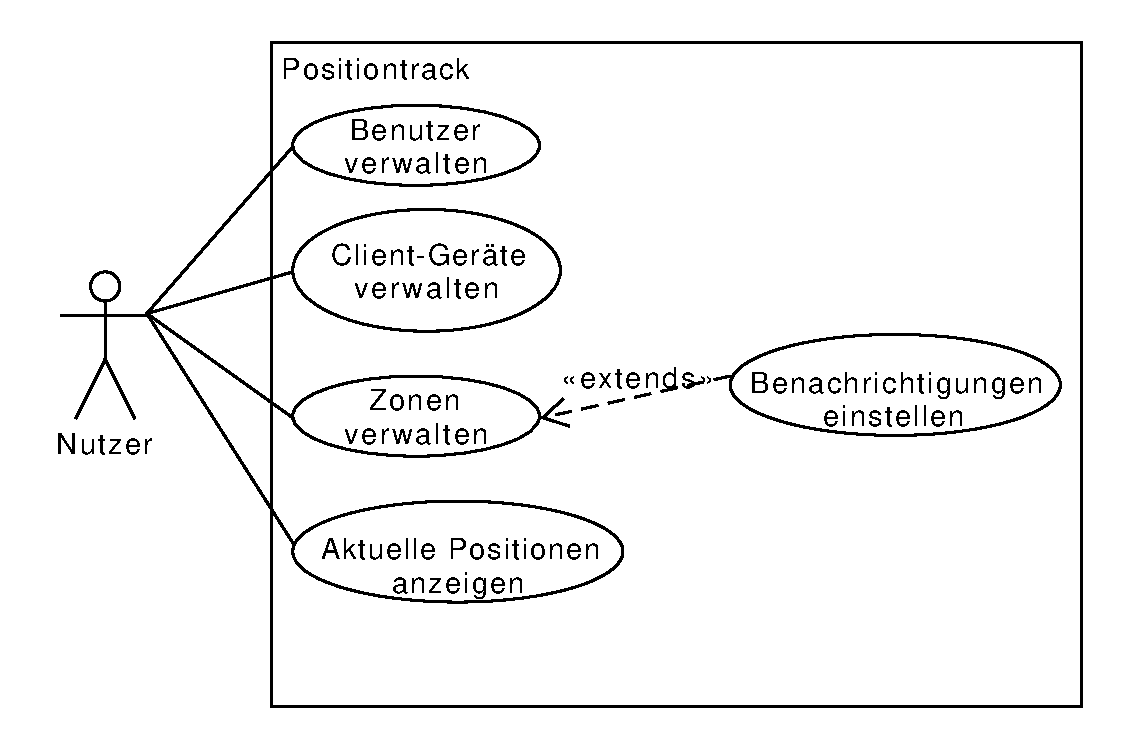
\includegraphics[scale=1]{images/useCaseDiagram.pdf}
\caption{caption}
\end{figure}

\subsubsection*{Benutzer verwalten}

\subsubsection*{Client-Geräte verwalten}

\subsubsection*{Zonen verwalten}

\subsubsection*{Aktuelle Positionen anzeigen}


\subsection{????Szenarien????}

\subsection{Systemanforderungen}
\begin{itemize}
\item Erfassen neuer Geräte und Nutzer
\item Rechteverwaltung zum Schutz der Daten
\item GeoFence Zonen Verwaltung
\item Zeitnahe Anzeige von neuen Positionen
\item Warnung beim Betreten/Verlassen von gesperrten Gebieten
\item Schnittstelle zur Datenerfassung
\item Management der Positionsdaten
\end{itemize}
\subsection{Architektur}

\subsection{Verwendete Technologien}

\section{Prototyp}
Erreichbarkeit, installation?

\section{Fazit}

%======================================================================
%   Literaturverzeichnis
%======================================================================
\renewcommand{\baselinestretch}{1.13}\normalsize
\markboth{BIBLIOGRAPHY}{BIBLIOGRAPHY}
\renewcommand{\bibname}{BIBLIOGRAPHY}
\bibliographystyle{plaindin}
\selectlanguage{ngerman}
\bibliography{literatur}
\cleardoublepage

%======================================================================
%   Selbstständigkeitserklärung
%======================================================================
\selectlanguage{ngerman}
\section*{Selbstständigkeitserklärung}
\thispagestyle{empty} Hiermit erklären wir, dass wir die vorliegende
Arbeit selbstständig angefertigt, nicht anderweitig zu
Prüfungszwecken vorgelegt und keine anderen als die angegebenen
Hilfsmittel verwendet haben. Sämtliche wissentlich verwendete
Textausschnitte, Zitate oder Inhalte anderer Verfasser
wurden ausdrücklich als solche gekennzeichnet.%\\[2ex]

\vspace{2cm}\noindent
%--------------------------------- \newline
\vspace{1cm}\noindent
--------------------------------- \newline
\vspace{1cm}\noindent
--------------------------------- \newline
\vspace{1cm}\noindent
--------------------------------- \newline
\vspace{1cm}\noindent

Görlitz, den 01. Dezember 2014

\end{document}